\documentclass{beamer}

\usetheme{Madrid}

\usepackage{graphicx}
\usepackage{amsmath}
\usepackage{amssymb}
\usepackage{booktabs}
\usepackage[ruled,vlined]{algorithm2e}
\usepackage{etoolbox}
\usepackage{tikz}
\usepackage{multicol}
\usetikzlibrary{shapes.geometric}

% Dummy commands for paper-specific macros
\newcommand{\pg}{\mathbf{p}}
\newcommand{\revision}[2]{#2}
\newcommand{\ieeeSmall}{}
\newcommand{\pegaseSmall}{}
\newcommand{\rteLarge}{}
\newcommand{\pegaseLarge}{}
\newcommand{\pegaseXLarge}{}
\newcommand{\gocXXL}{}

% Path to images from the paper folder
\graphicspath{{../paper/images/}}

\title{End-to-End Feasible Optimization Proxies for Large-Scale Economic Dispatch}
\author{Ilay Menachem}
\date{January 2026}

\begin{document}

\begin{frame}
    \titlepage
\end{frame}

% introduction
\section{Introduction}
\begin{frame}
    \frametitle{Motivation}
    \begin{itemize}
        \item \textbf{Trend:} Deep Learning for grid management and optimization
        \item \textbf{Challenge:} Respecting problem structure and constraints
        \item \textbf{Benefit:} Networks that respect constraints learn more efficiently and achieve better performance
    \end{itemize}
    
    \vspace{0.5cm}
    \begin{block}{The paper's contribution}
        A new closed-form method to make neural networks respect economic dispatch constraints \textit{by construction}
    \end{block}
\end{frame}

% previous works
\section{Previous Works}
\subsection{Optimization Proxies for OPF}
\begin{frame}
    \frametitle{Previous Works: Optimization Proxies}
    \begin{block}{Supervised Learning Approaches}
        \begin{itemize}
            \item Successfully applied to DC-OPF and AC-OPF
            % even in real-world grids, the grid topologies change frequently due to new construction and decommissioning of lines and transformers
            \item \textbf{Limitation:} Rely on fixed grid topologies
            \item Changes require expensive retraining and data re-generation
        \end{itemize}
    \end{block}
    
    \begin{block}{Graph Neural Networks}
        \begin{itemize}
            \item Can handle topology changes
            \item \textbf{Limitation:} Shown to be unstable on large-scale networks
        \end{itemize}
    \end{block}
\end{frame}

\subsection{Ensuring Feasibility}
\begin{frame}
    \frametitle{Previous Works: Ensuring Feasibility}
    \textbf{Problem:} ML proxies often violate physical constraints
    
    \vspace{0.3cm}
    \textbf{Existing Strategies:}
    \begin{itemize}
        \item \textbf{Active Set Learning:} Predict active constraints of the optimal solution (incorrect classifications $\rightarrow$ infeasibility)
        \item \textbf{Physics-Informed Models:} Add penalty terms for non-physical outputs (no feasibility guarantee)
        \item \textbf{Post-Processing:} Projection or power flow solvers to repair non-physical outputs (adds computational time)
        % this is the proposed approach but guarantees full feasibility if there is a feasible solution
        \item \textbf{End-to-End Layers:} Embed feasibility restoration (current methods fail to guarantee full feasibility or rely on restrictive assumptions)
    \end{itemize}
\end{frame}

\subsection{Scalability Challenges}
\begin{frame}
    \frametitle{Previous Works: Scalability Gap}
    \begin{alertblock}{Academic vs. Industrial Reality}
        \begin{itemize}
            \item Most research: small test systems ($<$ 300 buses)
            \item Real-world grids: tens of thousands of buses
        \end{itemize}
    \end{alertblock}
    
    \vspace{0.3cm}
    \begin{block}{The proposed approach}
        Test on large-scale systems up to 30,000 buses
    \end{block}
\end{frame}

% the economic dispatch problem
\section{The Economic Dispatch Problem}
\begin{frame}
    \frametitle{The Economic Dispatch Problem}
    \begin{block}{Objective}
        Minimize total production cost plus penalty for thermal limit violations:
        \[\min_{\boldsymbol{p}, \boldsymbol{r}, \boldsymbol{\xi}_{th}} c(\boldsymbol{p}) + M_{th} ||\boldsymbol{\xi}_{th}||_1\]
    \end{block}
    
    \begin{block}{Subject to:}
        \begin{itemize}
            \item $e^T\boldsymbol{p} = e^T\boldsymbol{d}$ (global power balance)
            \item $e^T\boldsymbol{r} \geq R$ (minimum reserve requirement)
            \item $\boldsymbol{p} + \boldsymbol{r} \leq \overline{\boldsymbol{p}}$ (generator output limits)
            \item $0 \leq \boldsymbol{p} \leq \overline{\boldsymbol{p}}$, $0 \leq \boldsymbol{r} \leq \overline{\boldsymbol{r}}$ (generator and reserve limits)
            \item $\underline{\boldsymbol{f}} - \boldsymbol{\xi}_{th} \leq \boldsymbol{\Phi}(\boldsymbol{p} - \boldsymbol{d}) \leq \overline{\boldsymbol{f}} + \boldsymbol{\xi}_{th}$ (thermal limits)
            \item $\boldsymbol{\xi}_{th} \geq 0$ (thermal limit violations non-negativity)
        \end{itemize}
    \end{block}
\end{frame}

% the proposed approach
\section{The Proposed Approach}
\begin{frame}
    \frametitle{End-to-End Learning with Feasibility Guarantee}
    \begin{center}
        \textbf{Key Idea:} Add specialized layers that guarantee feasibility by construction
    \end{center}
    
    \vspace{0.5cm}
    \begin{block}{Architecture Components}
        \begin{enumerate}
            \item Neural Network (predicts initial solution)
            \item Sigmoid Layer (enforces generator limits)
            \item Power Balance Repair Layer (enforces power balance)
            \item Reserve Repair Layer (enforces reserve requirements)
        \end{enumerate}
    \end{block}
    
    \vspace{0.3cm}
    \begin{alertblock}{Guarantee}
        If a feasible solution exists, the repair layers will output a feasible solution
    \end{alertblock}
\end{frame}

\subsection{Neural Network Architecture}
%% feed-forward architecture
\begin{frame}
    % the feed-forward in a red rectangle
    \begin{figure}[ht]
        \centering
        \includegraphics[width=0.85\linewidth]{figs/repair_layers.pdf}
    \end{figure}

    % purpose 
    \begin{alertblock}{Purpose}
        The feed-forward architecture is used to decide the $\boldsymbol{p}$ given the data.
    \end{alertblock}

    % we can use any type of neural network architecture maybe a good idea would be to use a GNN
\end{frame}

%% sigmoid layer
\subsection{Sigmoid Layer}
\begin{frame}
    % the sigmoid layer in a red rectangle
    \begin{figure}[ht]
        \centering
        \includegraphics[width=0.85\linewidth]{figs/repair_layers.pdf}
    \end{figure}

    % purpose 
    \begin{alertblock}{Purpose}
        The sigmoid layer is used to enforce the generator limits $0 \le \boldsymbol{p} \le \overline{\boldsymbol{p}}$.
    \end{alertblock}
\end{frame}

%% power balance layer
\subsection{Power Balance Layer}
\begin{frame}
    % the power balance layer in a red rectangle
    \begin{figure}[ht]
        \centering
        \includegraphics[width=0.85\linewidth]{figs/repair_layers.pdf}
    \end{figure}

    % purpose 
    \begin{alertblock}{Purpose}
        Assuming that the generator limits are respected, the power balance layer is used to enforce the power balance constraint $e^T\boldsymbol{p} = e^T\boldsymbol{d}$.
    \end{alertblock}
\end{frame}

\begin{frame}
    % illustration of the power balance layer
    \begin{figure}[ht]
    \centering
    \resizebox{0.42\columnwidth}{!}{
    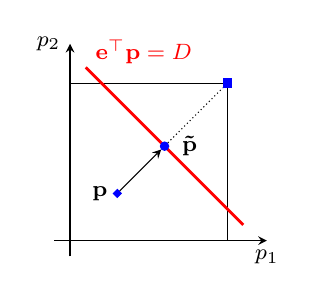
\begin{tikzpicture}[x=2cm,y=2cm]
        % X Axis
        \draw[black,-stealth] (-0.1, 0.0) -- (1.25, 0.0);
        \node[below] at (1.25, 0.0) {\footnotesize $p_{1}$};
        % Y axis
        \draw[black,-stealth] (0.0, -0.1) -- (0.0, 1.25);
        \node[left] at (0.0, 1.25) {\footnotesize $p_{2}$};
        
        % Unit hypercube
        \draw[black] (0,0) -- (0, 1) -- (1,1) -- (1,0) -- cycle;
        
        % Power balance constraint
        \draw[red,line width=1pt] (0.1, 1.1) -- (1.1, 0.1);
        \node[right, color=red] at (0.1, 1.2) {\footnotesize $\mathbf{e}^{\top}\pg = D$};
        
        % Max output
        \node[draw=blue, fill=blue, inner sep=0pt,minimum size=3pt] (p_bar) at (1.00, 1.00) {};
        % Prediction
        \node[diamond,draw=blue, fill=blue, inner sep=0pt,minimum size=3pt] (p_hat) at (0.30, 0.30) {};
        \node[left] at (0.3, 0.3) {\footnotesize $\pg$};
        % Feasible point
        \node[circle,draw=blue, fill=blue, inner sep=0pt,minimum size=3pt] (p_til) at (0.6, 0.6) {};
        \node[right] at (0.65, 0.6) {\footnotesize $\mathbf{{\tilde{p}}}$};
        
        % Proportional response visual
        \draw[black,-stealth] (p_hat) -- (p_til);
        \draw[black,densely dotted] (p_til) -- (p_bar);
    \end{tikzpicture}}
    \hfill
    \resizebox{0.42\columnwidth}{!}{
    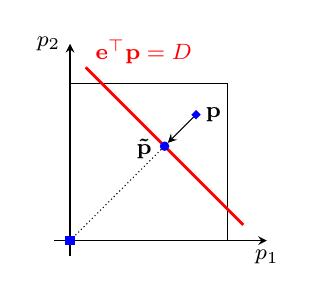
\begin{tikzpicture}[x=2cm,y=2cm]
        % X Axis
        \draw[black,-stealth] (-0.1, 0.0) -- (1.25, 0.0);
        \node[below] at (1.25, 0.0) {\footnotesize $p_{1}$};
        % Y axis
        \draw[black,-stealth] (0.0, -0.1) -- (0.0, 1.25);
        \node[left] at (0.0, 1.25) {\footnotesize $p_{2}$};
        
        % Unit hypercube
        \draw[black] (0,0) -- (0, 1) -- (1,1) -- (1,0) -- cycle;
        
        % Power balance constraint
        \draw[red,line width=1pt] (0.1, 1.1) -- (1.1, 0.1);
        \node[right, color=red] at (0.1, 1.2) {\footnotesize $\mathbf{e}^{\top}\pg = D$};
        
        % Min output
        \node[draw=blue, fill=blue, inner sep=0pt,minimum size=3pt] (p_bar) at (0.00, 0.00) {};
        % Prediction
        \node[diamond,draw=blue, fill=blue, inner sep=0pt,minimum size=3pt] (p_hat) at (0.80, 0.80) {};
        \node[right] at (0.8, 0.8) {\footnotesize $\pg$};
        % Feasible point
        \node[circle,draw=blue, fill=blue, inner sep=0pt,minimum size=3pt] (p_til) at (0.6, 0.6) {};
        \node[left] at (0.58, 0.58) {\footnotesize $\mathbf{{\tilde{p}}}$};
        
        % Proportional response visual
        \draw[black,-stealth] (p_hat) -- (p_til);
        \draw[black,densely dotted] (p_til) -- (p_bar);
    \end{tikzpicture}}
    \hfill\\
    \caption{%
        Illustration of the power balance layer with input $\pg$ and output $\mathbf{\tilde{p}}$.
        Left: $\mathbf{e}^{\top}\pg \, {<} \, D$ (energy shortage) and generators' dispatches are increased.
        Right: $\mathbf{e}^{\top}\pg \, {>} \, D$ (energy surplus) and generators' dispatches are decreased.
    }
    \label{fig:feasibility_layer:hypersimplex}
\end{figure}

\end{frame}

%% reserve layer
\subsection{Reserve Layer}
\begin{frame}
    % the reserve layer in a red rectangle
    \begin{figure}[ht]
        \centering
        \includegraphics[width=0.85\linewidth]{figs/repair_layers.pdf}
    \end{figure}

    % purpose 
    \begin{alertblock}{Purpose}
        Assuming that the power balance and generator limits are respected, the reserve layer is used to enforce the reserve requirement $e^T\boldsymbol{r} \geq R$.
    \end{alertblock}
\end{frame}

\begin{frame}
    % illustration of the reserve layer
    \begin{figure}[ht]
    \centering
    \resizebox{0.6\columnwidth}{!}{
    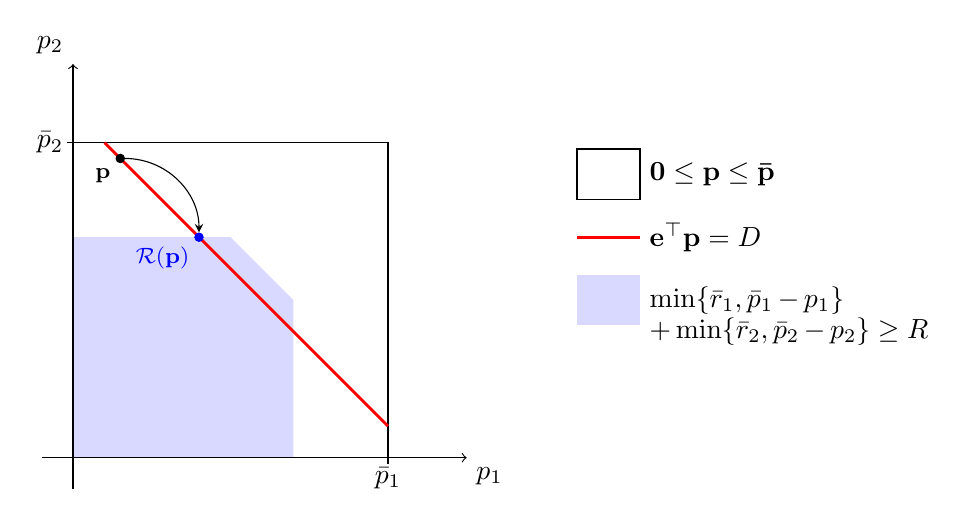
\begin{tikzpicture}[x=4cm,y=4cm]
        % X Axis
        \draw[black,->] (-0.1, 0.0) -- (1.25, 0.0);
        \node[below right] at (1.25, 0.0) {$p_{1}$};
            \draw[black] (1, -0.02) -- (1, 0.02);
            \node[below] at (1, 0.0) {$\bar{p}_{1}$};
        
        % Y axis
        \draw[black,->] (0.0, -0.1) -- (0.0, 1.25);
        \node[above left] at (0.0, 1.25) {$p_{2}$};
            \draw[black] (-0.02, 1) -- (+0.02, 1);
            \node[left] at (0, 1) {$\bar{p}_{2}$};
            
        % Reserve feasibility domain
        \fill[blue!50!white, fill opacity=0.3] (0,0) -- (0,0.7) -- (0.5, 0.7) -- (0.7, 0.5) -- (0.7, 0.0) -- cycle;
        
        % Domain of p1, p2
        \draw[black] (0,0) -- (0, 1) -- (1,1) -- (1,0) -- cycle;
        
        % Power balance constraint
        \draw[red,line width=1pt] (0.1, 1.0) -- (1.0, 0.1);
        
        % Infeasible prediction
        \node[circle,draw=black, fill=black, inner sep=0pt,minimum size=3pt] (phat_a) at (0.15, 0.95) {};
        \node[below left] at (0.15, 0.95) {\footnotesize $\pg$};
        
        % Feasible points of interest
        \node[circle,draw=blue, fill=blue, inner sep=0pt,minimum size=3pt] (pfeas1) at (0.4, 0.7) {};
        \node[below left, blue] at (0.4, 0.7) {\footnotesize $\mathcal{R}(\pg)$};
        
        \draw[-stealth] (phat_a.east) to [out=0,in=90] (pfeas1.north);
        
        % Legend
            % Domain of pg
            \draw[black] (1.6, 0.98) -- (1.8, 0.98) -- (1.8, 0.82) -- (1.6, 0.82) -- cycle;
            \node[right] at (1.8, 0.9) {$\mathbf{0} \leq \pg \leq \mathbf{\bar{p}}$};
            % Power Balance
            \draw[red, line width=1pt] (1.6, 0.7) -- (1.8, 0.7);
            \node[right] at (1.8, 0.7) {$\mathbf{e}^{\top} \pg = D$};
            % Reserve feasibility
            \fill[blue!50!white, fill opacity=0.3] (1.6, 0.58) -- (1.8, 0.58) -- (1.8, 0.42) -- (1.6, 0.42) -- cycle;
            \node[right] at (1.8, 0.5) {$\min\{\bar{r}_{1}, \bar{p}_{1} \, {-} \, p_{1}\}$};
            \node[right] at (1.8, 0.4) {$+\min\{\bar{r}_{2}, \bar{p}_{2} \, {-} \, p_{2}\} \geq R$};
    \end{tikzpicture}
    }
    \caption{Illustration of the reserve feasibility layer for $\mathbf{\bar{p}} {=} (1, 1)$, $\mathbf{\bar{r}}{=}(0.5, 0.5)$, $D {=} 1.1$, $R{=}0.8$ and the initial prediction $\pg {=} (0.15, 0.95)$. The recovered feasible dispatch is $\mathbf{\tilde{p}} {=} (0.4, 0.7)$.}
    \label{fig:feasibility_recovery:reserve}
\end{figure}

\end{frame}

%% what we got
\begin{frame}
    \frametitle{What we got?}
    what we got? \pause as much one can ask for! 
    % what we got
    \begin{itemize}
        \item ensure feasibility if there is a feasible solution
        \item informative gradients for the repair layers
        \item closed-form and simple $\rightarrow$ automatically differentiable
        \item closed-form and simple $\rightarrow$ fast
    \end{itemize}
\end{frame}

% the dataset
\section{Experimental Setup}
\subsection{Datasets}
\begin{frame}
    \frametitle{Datasets: Large-Scale Test Systems}    
    \begin{table}
        \centering
        \small
        \begin{tabular}{|l|c|c|c|}
            \hline
            \textbf{System} & \textbf{Buses} & \textbf{Generators} & \textbf{Branches} \\
            \hline
            ieee300 & 300 & 69 & 411 \\
            \hline
            pegase1k & 1,354 & 260 & 1,991 \\
            \hline
            rte6470 & 6,470 & 761 & 9,005 \\
            \hline
            pegase9k & 9,241 & 1,445 & 16,049 \\
            \hline
            pegase13k & 13,659 & 4,092 & 20,467 \\
            \hline
            goc30k & 30,000 & 3,526 & 35,393 \\
            \hline
        \end{tabular}
    \end{table}

    \pause
    \textbf{rte6470 is based on the full french grid!}
\end{frame}

% training
\subsection{Training}
\begin{frame}
    \frametitle{Training: Supervised and Self-Supervised}
    \begin{block}{Self-Supervised Learning}
        \begin{itemize}
            \item Train to minimize objective function and constraint penalties directly
            \item Eliminates need for labeled data and offline optimization
        \end{itemize}
    \end{block}
    \pause

    \begin{block}{Supervised Learning Loss}
        \[\mathcal{L}^{SL}(\hat{p}, p^*) = \underbrace{\frac{1}{|\mathcal{G}|} ||\hat{p} - p^*||_1}_{\text{MAE}} + \underbrace{\mu M_{th} ||\xi_{th}(\hat{p})||}_{\text{Thermal}} + \underbrace{\lambda \psi(\hat{p})}_{\text{Hard Constraints}}\]
    \end{block}
    
    \begin{block}{Self-Supervised Learning Loss}
        \[\mathcal{L}^{SSL}(p^*) = \underbrace{c(p^*)}_{\text{Cost}} + \underbrace{M_{th} \xi_{th}(p^*)}_{\text{Thermal}} + \underbrace{\lambda \psi(\hat{p})}_{\text{Hard Constraints}}\]
    \end{block}
    
    \begin{itemize}
        \item Hard constraints: $\psi(\hat{p}) = M_{pb}|e^T\boldsymbol{d} - e^T\hat{p}| + M_{r}\xi_{r}(\hat{p})$
    \end{itemize}
\end{frame}

% results
\section{Results}
\begin{frame}
    \frametitle{Experimental Results}
    \begin{block}{Key Findings}
        \begin{itemize}
            \item \textbf{E2ELR model outperformed all baselines} on every dataset
            \item \textbf{Same inference time} as unconstrained networks
        \end{itemize}
    \end{block}
    
    \begin{alertblock}{Impact}
        First method to guarantee full feasibility for large-scale economic dispatch while maintaining competitive speed and accuracy
    \end{alertblock}
\end{frame}

% conclusion
\section{Conclusion}
\begin{frame}<presentation:0>
    \frametitle{Conclusion}
    \begin{block}{Summary}
        \begin{itemize}
            \item Novel end-to-end architecture with repair layers
            \item Guarantees feasibility by construction (no post-processing)
            \item Closed-form, differentiable operations
            \item Successfully tested on systems up to 30,000 buses
            \item Superior performance compared to existing methods
        \end{itemize}
    \end{block}
\end{frame}

% end of presentation
\begin{frame}
    \frametitle{End of Presentation}
    \begin{center}
        \textbf{Thank you for your attention!}\\
        \vspace{1cm}
        \textbf{\Large{Questions?}}
        \vspace{1cm}
    \end{center}
\end{frame}

\end{document}